\newpage
\section{Plano de desenvolvimento}

	Implementamos e desenvolvemos essa aplicação durante nosso estudo com processamento de imagens e OCR (reconhecimento ótico de caracteres). Já está conseguindo reconhecer palavras completas com espaços e quebra de linhas. Assim conseguimos reconhecer qualquer letra ou palavras do nosso alfabeto, nosso projeto foi desenvolvido com o intuito de utilizar duas matérias muito importantes durante esse 6º módulo, que são Processamento de Imagem, e Sistema de Informação Inteligentes, dessas matérias retiramos conhecimento para o desenvolvimento dessa aplicação. 
	
	\begin{figure}[!htb]
		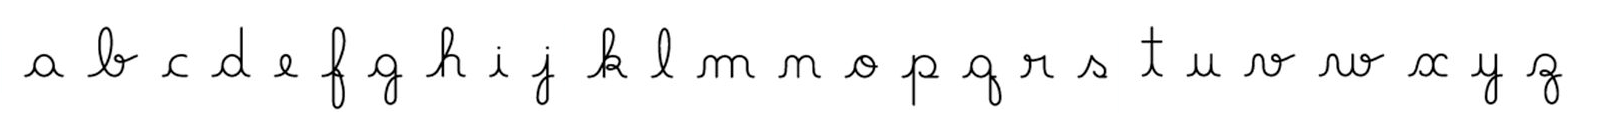
\includegraphics[scale=0.3]{alfa-manuscrito.png}
		\caption{Reconhecimento de letras manuscritas}
	\end{figure}
	
	A ideia é fazer o sistema reconhecer letras e palavras do alfabeto escrita a mão, para que funcionasse perfeitamente treinamos uma imagem do nosso alfabeto escrito a mão. Para que a aplicação aprenda todas as letras, e reconheça as palavras que forem escritas a mão, toda vez que quisermos que o sistema entenda uma palavra diferente, precisamos treiná-la, para que o sistema aprenda e com isso reconheça a palavra na imagem. O processo para que a aplicação leia a palavra, começa quando recortamos as letras do alfabeto que o sistema já reconhece e formamos a palavra, importamos para o programa para treiná-la, após o treinamento, pedimos para o sistema reconhecer a palavra que está na imagem, ele reconhece a palavra corretamente. Qualquer letra ou palavra do alfabeto que for colocado no sistema para reconhecimento, será reconhecida, no log do projeto é visualizado letra por letra a porcentagem de aprendizado do programa, assim verificamos como se fosse um gráfico para o aprendizado de cada letra que o programa teve, podendo ter uma ideia da qualidade do sistema que foi desenvolvido, até o momento todas palavras e letras foram reconhecidas com êxito.

	O programa reconhece basicamente todas as letras, e alguns símbolos, como traços, vírgula, ponto de exclamação, ponto de interrogação. Como na figura 4 abaixo treinamos esse alfabeto para testar o reconhecimento.
	
	\begin{figure}[!htb]
		\centering
		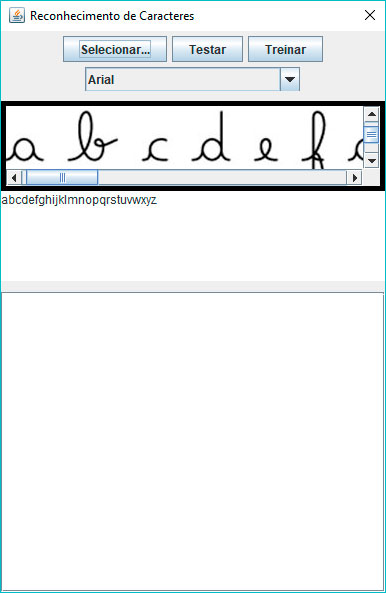
\includegraphics[width=.5\linewidth]{02-aprender-alfabeto-manuscrito.jpg} 
		\caption{Importando alfabeto} 
	\end{figure} 
	
	Após selecionar a imagem do alfabeto, clicamos em treinar, assim a aplicação executa o treinamento daquela imagem, para o reconhecimento das letras, como mostra na figura 5.
	
	\begin{figure}[!htb]
		\centering
		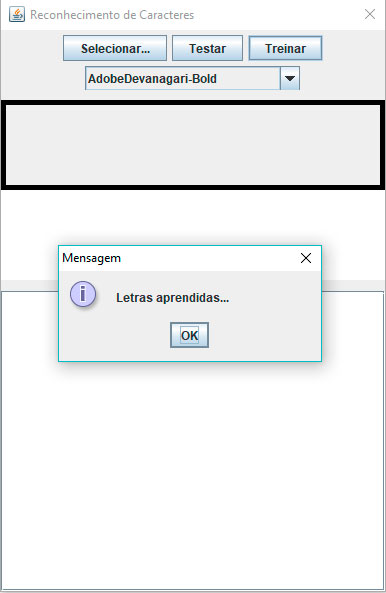
\includegraphics[scale=0.5]{03-sistema-aprendeu-as-letras.jpg}
		\caption{Aprendizado das letras}
	\end{figure}
	
	Já na figura 6 importamos as letras que desejamos que o programa reconheça.
	
	\begin{figure}[!htb]
		\centering
		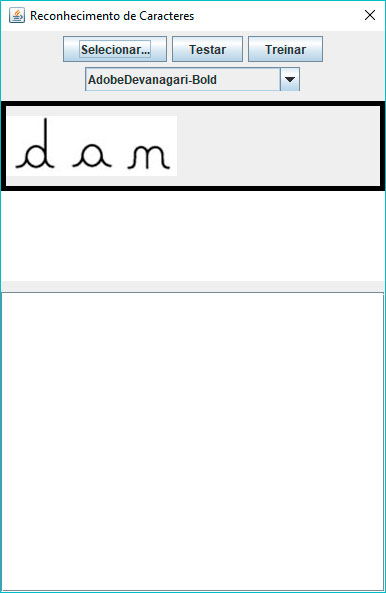
\includegraphics[scale=0.5]{04-introduzir-a-imagem-para-ser-reconhecida.jpg}
		\caption{Importando as letras que serão reconhecidas}
	\end{figure}
	
	Por fim, na figura 7 o programa mostra o relatório de de reconhecimento aproximado e o resultado da análise.
	
	\begin{figure}[!htb]
		\centering
		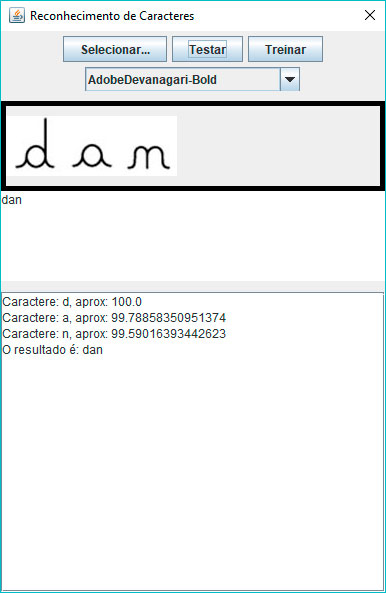
\includegraphics[scale=0.5]{05-imagem-reconhecida-resultado-esperado.jpg}
		\caption{Relatório de reconhecimento das letras}
	\end{figure}

	O projeto foi desenvolvido com êxito, obtemos algumas falhas ao longo desse processo, como treinar a letra ou palavra utilizada, mas conseguimos resolver o problema buscando algumas informações de redes neurais, e após o entendimento de algumas regras, conseguimos normalizar o código que está sendo executado completamente.